\documentclass{article}
%\usepackage{geometry}
%\geometry{top = 1in, bottom = 1in, left = 1in, right = 1in}
\usepackage[top = 0.7in, bottom = 0.7in, left = 0.7in, right = 0.7in]{geometry}
\usepackage{amsmath,amssymb,amsthm,mathrsfs}
\usepackage{graphicx}
\usepackage{bm}
\usepackage{float}
\usepackage[font=footnotesize,labelfont=bf]{caption}
\usepackage{movie15}
\usepackage{hyperref}

\usepackage{fancyhdr}
\pagestyle{fancy}
\rhead{\footnotesize {09/17/2012 ; MESA version 4299} }
\chead{\footnotesize {Authors: Jared Brooks, Lars Bildsten, Bill Paxton} }
\lhead{\footnotesize {mesa/star/test\_suite/1M\_thermohaline} }

\begin{document}
	
	\begin{center}
	  \begin{Large}
	    \textbf{1M THERMOHALINE}\\
	  \end{Large}
	\end{center}

        This test is to show the capability of \texttt{MESA} to allow mixing through thermohaline convection.  It evolves a 1 $M_\odot$ ZAMS star through the main sequence and up the RGB and cuts off when the hydrogen boundary mass grows to 0.238 (\texttt{h1\_boundary\_mass\_limit = 0.238}).  This means that all of the cells interior to the mass coordinate 0.238 have a hydrogen mass fraction less than $10^{-4}$ (essentially, the core is depleted of hydrogen).  To verify that this test ran successfully, \texttt{MESA} checks a set of parameters to see if they fall inside a range of expected values, listed in \texttt{src/run\_star\_extras.f}.  If all the parameter values fall within their respective ranges, the terminal output at the end of the run should read \texttt{``all values are within tolerances''}.\\

        There are a number of important inlist controls to allow the star to undergo thermohaline convection.  Here are the controls in the \texttt{\&star\_job} section that relate to velocity and rotation:

        \begin{itemize}
        \item \texttt{change\_v\_flag = .true.}
        \item \texttt{new\_v\_flag = .true.}
        \item \texttt{change\_rotation\_flag = .true.}
        \item \texttt{new\_rotation\_flag = .true.}
        \item \texttt{set\_initial\_surface\_rotation\_v = .true.}
        \item \texttt{new\_surface\_rotation\_v = 10 ! km/sec    for 1.0 M}
        \end{itemize}

        The \texttt{\&controls} section of the inlist also contains controls necessary for thermohaline convection.  It turns on Ledoux criterion and sets a smoothing control (\texttt{use\_Ledoux\_criterion = .true. ; nsmooth\_gradL\_composition\_term = 1}), uses hydrogen mass fraction to compute $\nabla{_\mu}$ (\texttt{use\_gradmu\_X\_for\_mlt = .true.}), and sets a minimum number of iterations in newton for hydro solve (\texttt{newton\_itermin = 2}).  It also sets the weight of the omega function (\texttt{omega\_function\_weight = 20 ! omega\_function = omega\_function\_weight*log10(omega)}) and the effect of rotation on mass loss (\texttt{mdot\_omega\_power = 0.43 ! Mdot = Mdot\_no\_rotation/(1 - Osurf/Osurf\_crit)\^mdot\_omega\_power}).  Most importantly, it sets the efficiency of mixing from semiconvection (\texttt{alpha\_semiconvection = 4d-2}) and thermohaline convection (\texttt{thermo\_haline\_coeff = 2}).\\

        The star's main sequence and initial climb up the RGB can be seen in the HR-diagram to the left (figure \ref{fig:1}).  To the right is an abundance profile from the start of the run (figure \ref{fig:2}).

        \begin{figure}[H]
          \begin{minipage}[b]{0.5\linewidth}
	    \centering
	    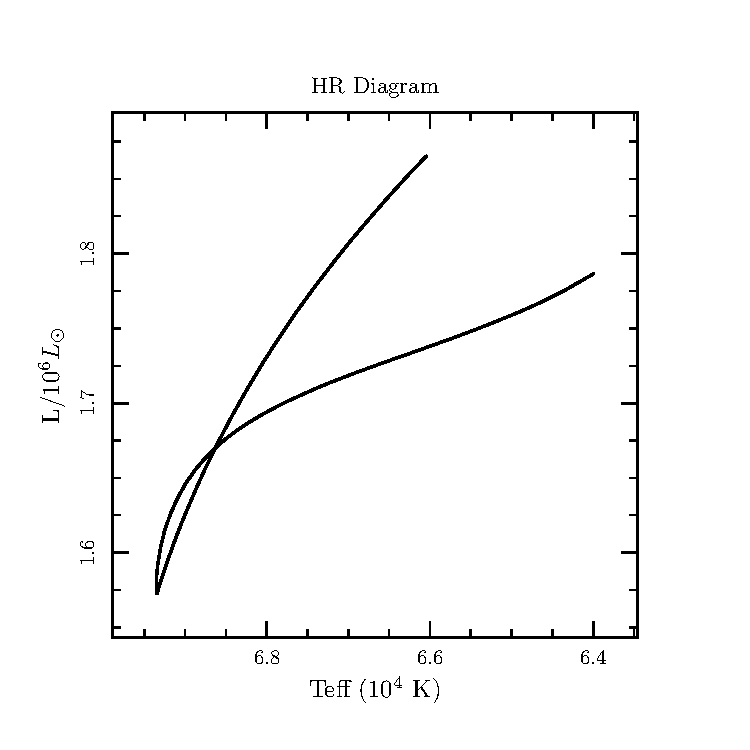
\includegraphics[width = 3.8in]{/Users/jaredbrooks/1M_thermohaline/plots_out/HR_Diagram.pdf}
	    \caption{HR-diagram shows main sequence and climb up RGB}
	    \label{fig:1}
          \end{minipage}
          \hspace{0cm}
          \begin{minipage}[b]{0.5\linewidth}
            \centering
            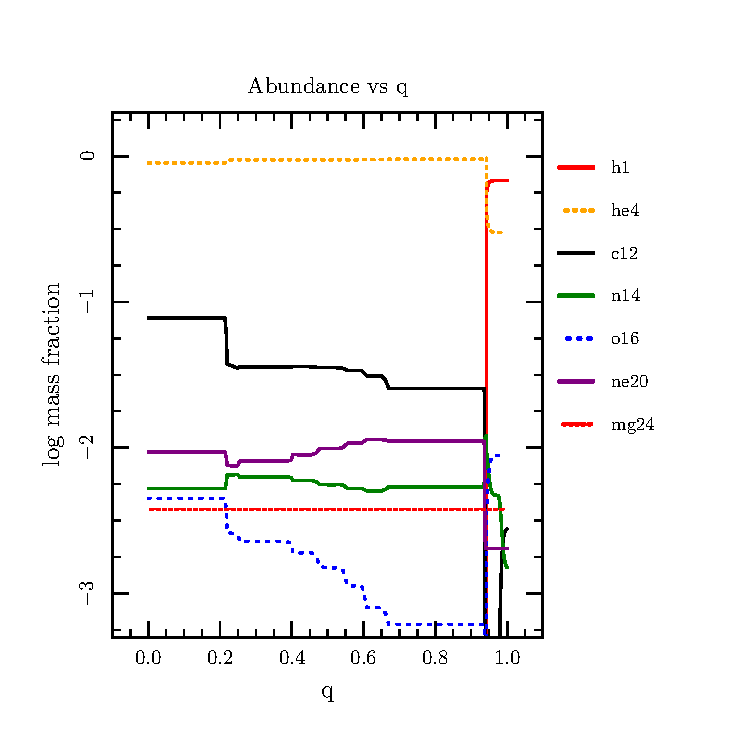
\includegraphics[width = 3.8in]{/Users/jaredbrooks/1M_thermohaline/plots_out/Abundance_vs_q_1.pdf}
            \caption{Abundance profile at start of run}
            \label{fig:2}
          \end{minipage}
	\end{figure}

        \pagebreak

        Below are two profiles from the end of the run, both plotted against q with the same range, where q is the fraction of star mass interior to outer boundary of each zone, moving outwards from the core.  The range shown is just below the main convection zone and right on top of the core.  This small range is the only place in the star (besides the outer envelope) where $\nabla{_\mu}$ goes negative and allows for thermohaline convection.  The profile on the left (figure \ref{fig:3}) shows $\nabla{_\mu}$ and the profile on the right (figure \ref{fig:4}) shows 1/$\mu$ along with temperature.

        \begin{figure}[H]
          \begin{minipage}[b]{0.5\linewidth}
            \centering
            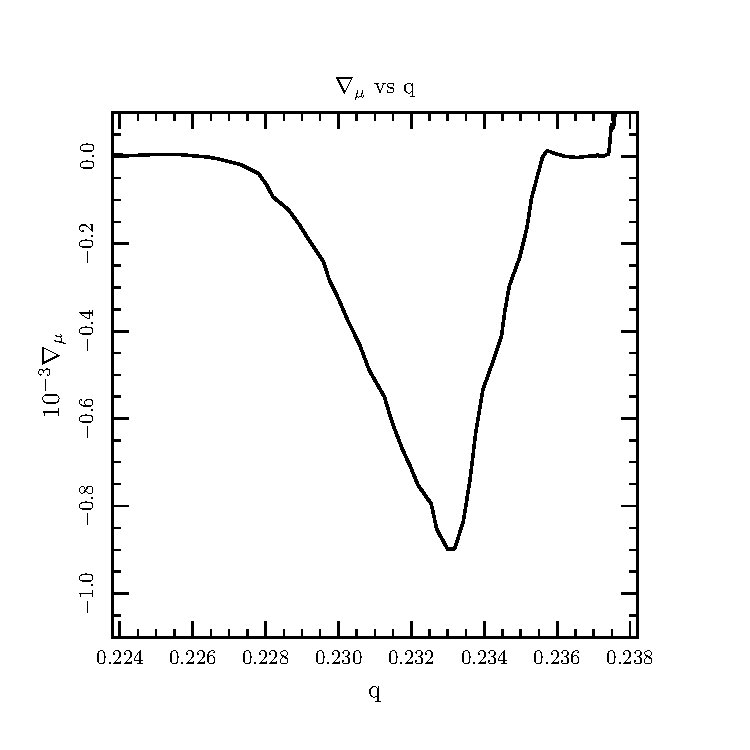
\includegraphics[width = 3.8in]{/Users/jaredbrooks/1M_thermohaline/plots_out/Grad_vs_q.pdf}
            \caption{Profile of $\nabla{_\mu}$ just below convection zone}
            \label{fig:3}
          \end{minipage}
          \hspace{0cm}
          \begin{minipage}[b]{0.5\linewidth}
            \centering
            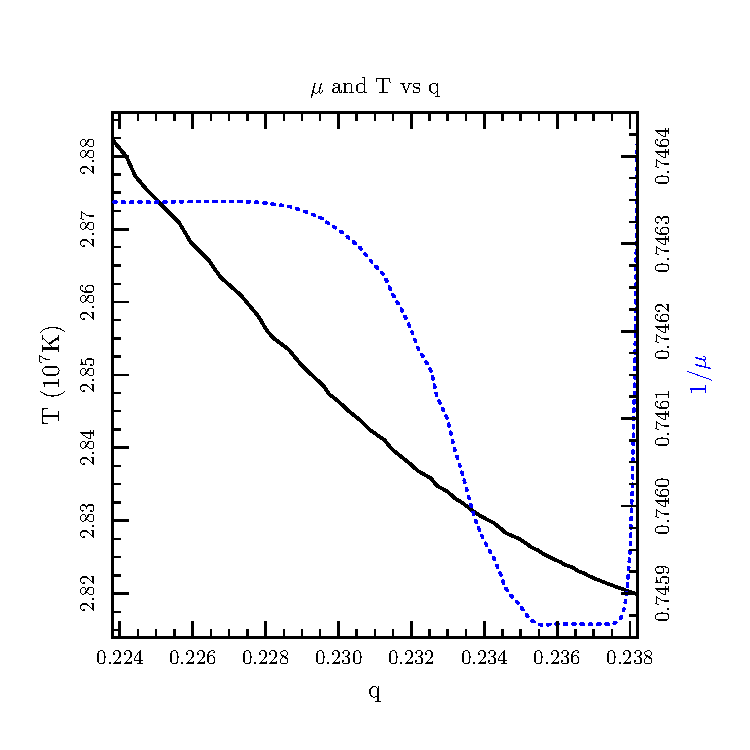
\includegraphics[width = 3.8in]{/Users/jaredbrooks/1M_thermohaline/plots_out/mu_vs_q.pdf}
            \caption{Profile of 1/$\mu$ and temperature just below convection zone}
            \label{fig:4}
          \end{minipage}
        \end{figure}

        \pagebreak

        Below is a video showing changes in mixing coefficients plotted against m/$M_\odot$.  The number at the top-right is the model number.  The run reaches 12 Gyr at about model number 300.  Click the figure to begin the video, double click to replay (must be using adobe reader to view movie).  Below that is a mixing coefficients profile taken from the end of the run (figure \ref{fig:6}).

        \begin{figure}[H]
          \includemovie[poster,text={\small(Loading Video...)}]{18cm}{15cm}{mixing.mp4}
        \end{figure}

        \begin{figure}[H]
          \centering
          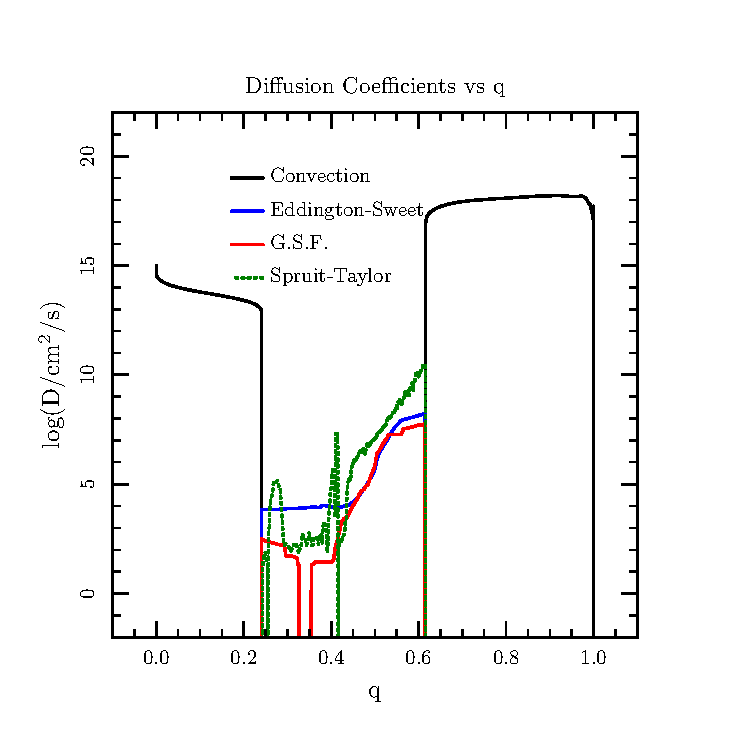
\includegraphics[width = 5in]{/Users/jaredbrooks/1M_thermohaline/plots_out/Diffusion_Coefficients_vs_q.pdf}
          \caption{Mixing coefficients from the end of the run, thermohaline at bottom of convection zone}
          \label{fig:6}
        \end{figure}

        \pagebreak

        To the left is a plot (figure \ref{fig:8}) showing the evolution of the thermohaline convection zone for the last 1.4 Gyr in blue, bordered by the bottom of the main convection zone in black.  To the right (figure \ref{fig:9}) is an abundance profile from the end of the run, showing the composition boundary just above the thermohaline convection zone.

        \begin{figure}[H]
          \begin{minipage}[b]{0.5\linewidth}
            \centering
            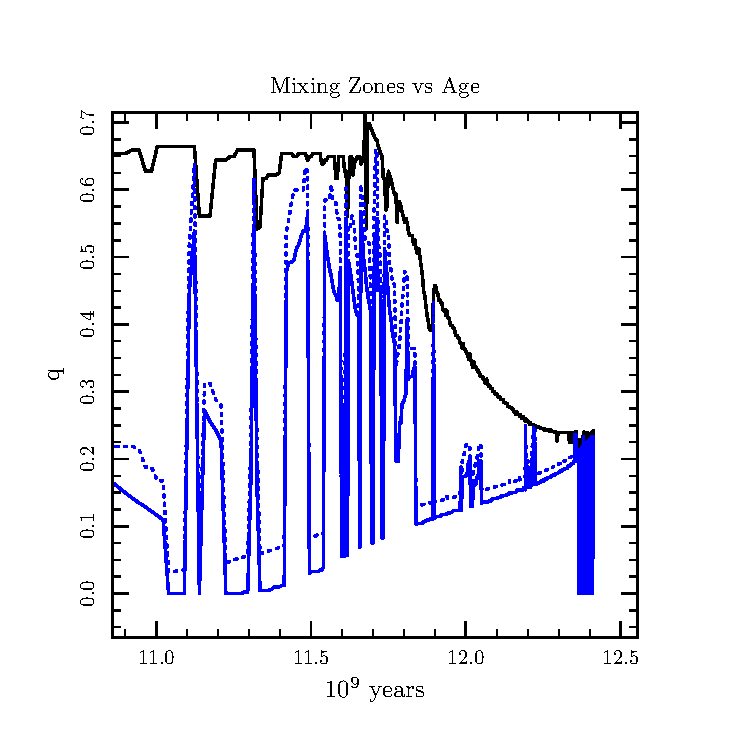
\includegraphics[width = 3.8in]{/Users/jaredbrooks/1M_thermohaline/plots_out/Mixing_vs_Age.pdf}
            \caption{Blue thermohaline convection zone bordered by bottom of main convection zone in black}
            \label{fig:8}
          \end{minipage}
          \hspace{0cm}
          \begin{minipage}[b]{0.5\linewidth}
            \centering
            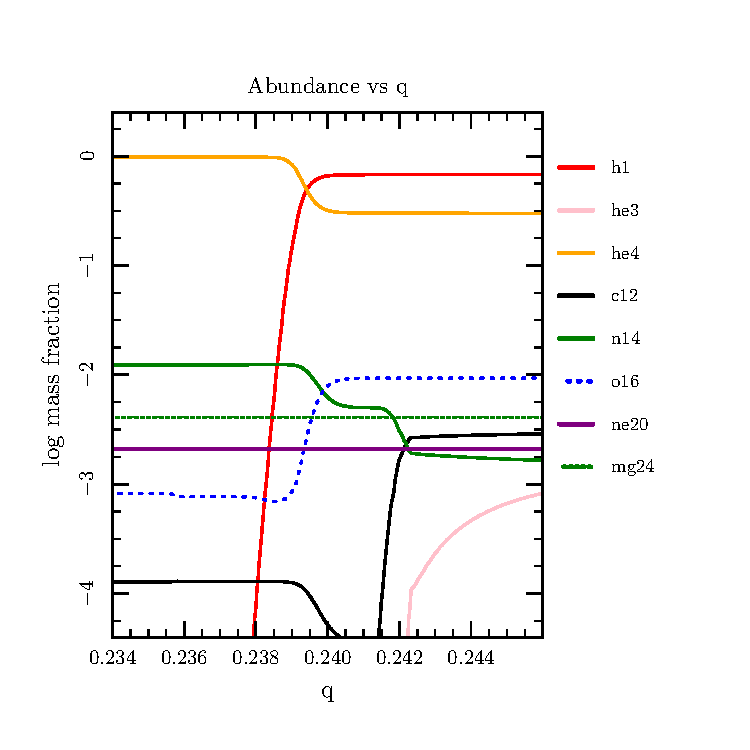
\includegraphics[width = 3.8in]{/Users/jaredbrooks/1M_thermohaline/plots_out/Abundance_vs_q_83.pdf}
            \caption{Composition boundary just above thermohaline at end of run}
            \label{fig:9}
          \end{minipage}
        \end{figure}

        \pagebreak

        This final plot (figure \ref{fig:7}) shows a few internal \texttt{MESA} variables, such as the size of the time-step, the number of zones, and the number of retries against the model number in order to give some understanding of how hard \texttt{MESA} is working throughout the run and where some areas of problems/interest might be.

        \begin{figure}[H]
          \centering
          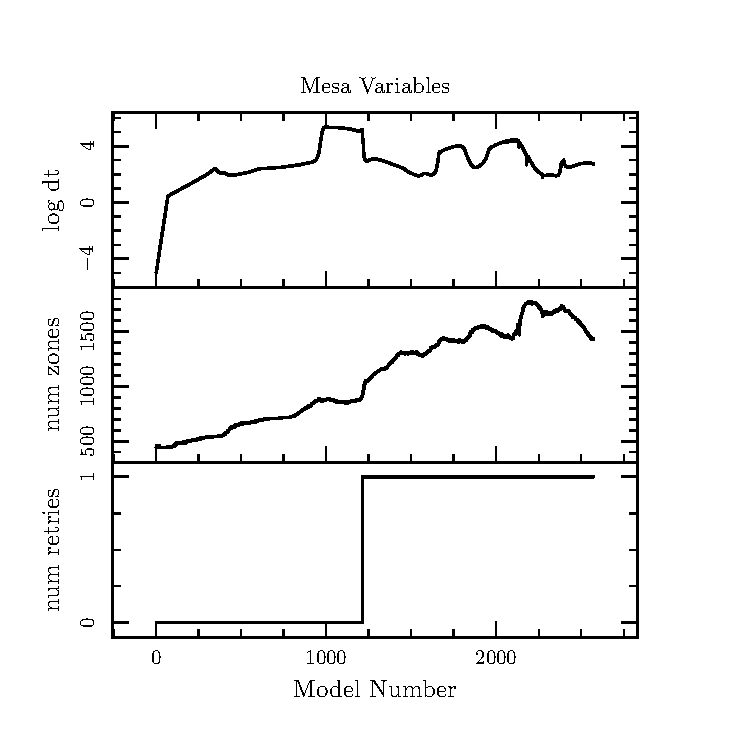
\includegraphics[width = 5in]{/Users/jaredbrooks/1M_thermohaline/plots_out/Mesa_Variables.pdf}
          \caption{\texttt{MESA} variables plotted against model number show how hard \texttt{MESA} is working}
          \label{fig:7}
        \end{figure}

\end{document}
